\begin{frame}
    \begin{theorem}{Upper bound for k=3}
        \[D(n,3)=\Omega(n^2/e^{O(\sqrt{\log n})})\]
    \end{theorem}
    \begin{heading}{Outline of the proof:}
    \begin{itemize}
        \item We will construct a graph whose reconfiguration graph is the disjoint union of \(n/e^{o(\sqrt{\log n})}\) paths of linear length
        \item We prove that we can add not many vertices to this graph to connect it and make the diameter sum of the components.
    \end{itemize}
    \end{heading}
\end{frame}

%--------------------------------------------

\begin{frame}{AP-Free}
    Set of integers is 3-AP free if it does not contain arithmetic progression of length 3, \(s_1<s_2<s_3\) such that:
    \[s_2-s_1=s_3-s_2\]
    If \(S\) is AP free then \(4S+1\) is as well.\\
    \pause
    \begin{theorem}{Theorem}
        There exists 3-AP subset of \(n\) of size \(n/e^{o(\sqrt{\log n})}\). \framemark
    \end{theorem}
    There is 3-AP subset of [\(1,\dots,n\)] only containing values where \(v=1 \text{ mod } 4\) of~size~\(n/e^{o(\sqrt{\log n})}\) (odd 3-AP-free sequence)
\framereference{A.~Behrend, \emph{On sets of integers which contain no three terms in arithmetical progression}, Proceedings of the National Academy of Sciences, 32(12):331--332, 1946.}
\end{frame}

%--------------------------------------------

\begin{frame}
\begin{lemma}{Lemma}
    Let \(n\) be a prime number and \(S\) be an odd 3 AP free sequence where maximum integer is at most \(n/8\). Then, there exists a graph on \(n-1\) vertices whose reconfiguration graph is the disjoint union of \(|S|\) paths of length \(n-3\).
\end{lemma}
\onslide<2>{
    We start from a clique on \(n\) vertices, and remove edges \((i,i+s)\), \((i+2s)\).
}
\begin{figure}
    \centering
    \begin{tikzpicture}[scale=1]

    \node[circle, draw=black, fill=white, minimum size=0.6cm, line width=1.5pt] (p0) at (0, 0) {$0$};
    \node[circle, draw=black, fill=white, minimum size=0.6cm, line width=1.5pt] (p1) at (1, 0) {$1$};
    \node[circle, draw=black, fill=white, minimum size=0.6cm, line width=1.5pt] (p2) at (2, 0) {$2$};
    \node[circle, draw=black, fill=white, minimum size=0.6cm, line width=1.5pt] (p3) at (3, 0) {$3$};
    \node[circle, draw=black, fill=white, minimum size=0.6cm, line width=1.5pt] (p4) at (4, 0) {$4$};
    \node[circle, draw=black, fill=white, minimum size=0.6cm, line width=1.5pt] (p5) at (5, 0) {$5$};
    \node[circle, draw=black, fill=white, minimum size=0.6cm, line width=1.5pt] (p6) at (6, 0) {$6$};
    \node[circle, draw=black, fill=white, minimum size=0.6cm, line width=1.5pt] (p7) at (7, 0) {$7$};
    \node[circle, draw=black, fill=white, minimum size=0.6cm, line width=1.5pt] (p8) at (8, 0) {$8$};
    \node[circle, draw=black, fill=white, minimum size=0.6cm, line width=1.5pt] (p9) at (9, 0) {$9$};
    \node[circle, draw=black, fill=white, minimum size=0.6cm, line width=1.5pt] (p10) at (10, 0) {$10$};

    \onslide<2>{
        \draw[line width=1.5pt, bend left=30, dashed] (p0) to (p3);
        \draw[line width=1.5pt, bend left=35, dashed] (p0) to (p6);
        \draw[line width=1.5pt, bend left=30, dashed] (p3) to (p6);
        \draw[line width=1.5pt, bend left=35, dashed] (p3) to (p9);
        \draw[line width=1.5pt, bend left=30, dashed] (p6) to (p9);
    
        \fill[cfblue] (0, -0.5) circle (0.1);
        \fill[cfblue] (2.9, -0.5) circle (0.1);
        \fill[cfblue] (5.9, -0.5) circle (0.1);
        \fill[cfpink] (3.1, -0.5) circle (0.1);
        \fill[cfpink] (6.1, -0.5) circle (0.1);
        \fill[cfpink] (9, -0.5) circle (0.1);
    }
\end{tikzpicture}

\end{figure}
\pause
 \(n\) is prime, thus each \(s\) gives us an induced cycle.
\end{frame}

%--------------------------------------------

\begin{frame}
    \begin{heading}{\(R_3(G)\) only contains vertices of the form \((i, i+s, i+2s)\)}
        Consider independent set \(\set{a,b,c}\) : \ \(a<b<c\), where
        \[b-a=x \qquad c-b=y \qquad c-a=z\]\\
        \(\{x,y,z\} \in \ S \cup 2S\) thus they are either 1 or 2 mod 4.\\
        but \(z=x+y\) thus \(x,y \in S, \ z \in 2S\)  \\
        \pause
        \[x=s \qquad y=s' \qquad z=2s''\]\\
        This would mean that \(2s''=s+s'\), but \(S\) is 3AP-Free thus \(s=s'=s''\).
    \end{heading}
\end{frame}

%--------------------------------------------

\begin{frame}{}
\begin{heading}{Cycles are induced - There is no edge connecting the cycles.}

    Sets in each cycle contains vertices 
    \(\set{i,i+s, i+2s}\).\\
    
    \vspace{1em}
    
    Consider two sets from different cycles 
    
    \vspace{-1em}
    
    \[I=\set{a,a+s,a+2s}, I'=\set{a',a'+s', a'+2s'}\]
    If \(I \cap I'=\set{x,y}\) then 
    \[x-y \text{ mod n } \in \set{\pm s, \pm 2s} \cap \set{\pm s', \pm 2s'}\]
    not possible as \(s,s' < n/8\) and are \(1 \text{ mod } 4\).
    \vspace{-0.5em}
    \begin{figure}
        \centering
        
\begin{tikzpicture}[scale=0.9]
    \node[circle, draw=black, fill=cfgr, minimum size=0.6cm, line width=1.5pt] (p0) at (0, 0) {$0$};
    \node[circle, draw=black, fill=cfred, minimum size=0.6cm, line width=1.5pt] (p1) at (1, 0) {$1$};
    \node[circle, draw=black, fill=white, minimum size=0.6cm, line width=1.5pt] (p2) at (2, 0) {$2$};
    \node[circle, draw=black, fill=cfgr, minimum size=0.6cm, line width=1.5pt] (p3) at (3, 0) {$3$};
    \node[circle, draw=black, fill=white, minimum size=0.6cm, line width=1.5pt] (p4) at (4, 0) {$4$};
    \node[circle, draw=black, fill=cfred, minimum size=0.6cm, line width=1.5pt] (p5) at (5, 0) {$5$};
    \node[circle, draw=black, fill=cfgr, minimum size=0.6cm, line width=1.5pt] (p6) at (6, 0) {$6$};
    \node[circle, draw=black, fill=white, minimum size=0.6cm, line width=1.5pt] (p7) at (7, 0) {$7$};
    \node[circle, draw=black, fill=white, minimum size=0.6cm, line width=1.5pt] (p8) at (8, 0) {$8$};
    \node[
      circle,
      draw=black,
      minimum size=0.6cm,
      line width=1.5pt,
      path picture={
        \fill[cfgr]
          (path picture bounding box.center) ++(90:0.3cm)
          arc (90:270:0.3cm) -- cycle;
        \fill[cfred]
          (path picture bounding box.center) ++(-90:0.3cm)
          arc (-90:90:0.3cm) -- cycle;
      }
    ] (p9) at (9,0) {$9$};
    \node[circle, draw=black, fill=white, minimum size=0.6cm, line width=1.5pt] (p8) at (10, 0) {$10$};

    \draw[line width=1.5pt, bend left=35, dashed] (p0) to (p3);
    \draw[line width=1.5pt, bend left=35, dashed] (p0) to (p6);
    \draw[line width=1.5pt, bend left=35, dashed] (p3) to (p6);
    \draw[line width=1.5pt, bend left=35, dashed] (p3) to (p9);
    \draw[line width=1.5pt, bend left=35, dashed] (p6) to (p9);

    \draw[line width=1.5pt, bend right=35, dashed] (p1) to (p5);
    \draw[line width=1.5pt, bend right=35, dashed] (p1) to (p9);
    \draw[line width=1.5pt, bend right=35,dashed] (p5) to (p9);
\end{tikzpicture}

    \end{figure}
    \end{heading}
\end{frame}

%--------------------------------------------

\begin{frame}{}
    We have shown that we can obtain a graph which is a union of \(|S|\) cycles of length \(n\).\\
    \pause
    \vspace{1em}
    Now, we remove vertex \(0\) from the graph, each cycle becomes a path. \\
    \pause
    \vspace{1em}
    Every cycle contained two sets containing \(0\), thus length of the paths is \(n-3\).
    \pause
    \begin{lemma}{Lemma}
    Let \(n\) be a prime number and \(S\) be an odd 3 AP free sequence where maximum integer is at most \(n/8\). Then, there exists a graph on \(n-1\) vertices whose reconfiguration graph is the disjoint union of \(|S|\) paths of length \(n-3\).
    \end{lemma}
\end{frame}

%--------------------------------------------

\begin{frame}{}
    \begin{lemma}{Lemma}
        Let \(n\) be a prime number and \(S\) be an odd 3 AP free sequence where maximum integer is at most \(n/8\). Then, there exists a graph on \(n-1\) vertices whose reconfiguration graph is the disjoint union of \(|S|\) paths of length \(n-3\).
    \end{lemma}
    \begin{theorem}{Theorem}
        There exists 3-AP subset of \(n\) of size \(n/e^{o(\sqrt{\log n})}\).
    \end{theorem}   
    \pause
    \begin{lemma}{Lemma}
        For a prime number \(n\) there exists a graph on \(n-1\) vertices whose configuration graph is the disjoint union of \(O(n/e^{o(\sqrt{\log n})})\) paths of length \(n-3\).
    \end{lemma}
\end{frame}

%--------------------------------------------

\begin{frame}{}
    \begin{lemma}{Gluing Lemma}
        Let \(k \geq 3\). Let \(G\) be a graph on \(n\) vertices whose \(k\)-configuration graph contains \(r\) connected components. Then, there exists a graph on at most \(n+(3k-2)\cdot (r-1)\) vertices whose configuration graph had diameter at least \((4k-2)(r-1)+\sum d_i\)
    \end{lemma}
    \begin{heading}{Proof overview}
        \begin{itemize}
            \item We connect disjoint paths \(i, \ i+1\) by adding \(3k-2\)  vertices to connect last set in \(i\) with first set in \(i+1\).
  
        \end{itemize}
    \end{heading}
\end{frame}

%--------------------------------------------

\begin{frame}{}
\begin{columns}
    \begin{column}{0.8\textwidth}
        \begin{heading}{Symbols}
            \begin{itemize}
                \item \(B=\set{b_1,b_2,b_3}\) - last independent set in path \(i\)
                \item \(A=\set{a_1,a_2,a_3}\) - first independent set in path \(i+1\)
                \item \(b_1\) - last vertex modified to obtain \(B\) in path \(i\)
                \item \(a_3\) - first vertex modified in path \(i+1\)
            \end{itemize}
        \end{heading}
        \onslide<2->{
        \begin{heading}{Construction}
        \begin{itemize}
            \item we add \(3k-2\) new vertices \(x_i\) and connect them with everything
            \onslide<3->{
            \item remove vertices \((x_i,\ x_j)\) for \(|i-j|<k\)
            }
            \onslide<4->{
            \item remove vertices \((x_i,b_j)\), \((x_{3k-2-i}, a_{k-j})\) for \(j>i\)
            }
        \end{itemize}
        \end{heading}
        }
    \end{column}
    \begin{column}{0.3\textwidth}
        \begin{figure}
            \centering
            \begin{tikzpicture}[scale=0.85]
\coordinate (a0) at (2,0);
\coordinate (a1) at (1,0);
\coordinate (a2) at (0,0);

\coordinate (b0) at (2,8);
\coordinate (b1) at (1,8);
\coordinate (b2) at (0,8);

\coordinate (x1) at (3,1);
\coordinate (x2) at (3,2);
\coordinate (x3) at (3,3);
\coordinate (x4) at (3,4);
\coordinate (x5) at (3,5);
\coordinate (x6) at (3,6);
\coordinate (x7) at (3,7);
\coordinate (x8) at (3,8);

\draw[line width=1.5pt, dashed] (a0) to (a1);
\draw[line width=1.5pt, dashed] (a1) to (a2);
\draw[line width=1.5pt, bend left=90, dashed] (a0) to (a2);

\draw[line width=1.5pt, dashed] (b0) to (b1);
\draw[line width=1.5pt, dashed] (b1) to (b2);
\draw[line width=1.5pt, bend right=90, dashed] (b0) to (b2);

\only<3->{
    \draw[line width=1.5pt, dashed] (x1) to (x2);
    \draw[line width=1.5pt, dashed] (x2) to (x3);
    \draw[line width=1.5pt, dashed] (x3) to (x4);
    \draw[line width=1.5pt, dashed] (x4) to (x5);
    \draw[line width=1.5pt, dashed] (x5) to (x6);
    \draw[line width=1.5pt, dashed] (x6) to (x7);

    \draw[line width=1.5pt, bend right=90, dashed] (x1) to (x3);
    \draw[line width=1.5pt, bend left=90, dashed] (x2) to (x4);
    \draw[line width=1.5pt, bend right=90, dashed] (x3) to (x5);
    \draw[line width=1.5pt, bend left=90, dashed] (x4) to (x6);
    \draw[line width=1.5pt, bend right=90, dashed] (x5) to (x7);
}
\only<4->{
    \draw[line width=1.5pt, dashed] (a0) to (x1);
    \draw[line width=1.5pt, bend left=40, dashed] (a0) to (x2);
    \draw[line width=1.5pt, bend left=30, dashed] (a1) to (x1);

    \draw[line width=1.5pt, dashed] (b0) to (x7);
    \draw[line width=1.5pt, bend right=40, dashed] (b0) to (x6);
    \draw[line width=1.5pt, bend right=30,dashed] (b1) to (x7);
}

\only<1>{
    \node[circle, draw=black, fill=white, line width=1.5pt, font=\footnotesize] at (a2)  {$a_{3}$};
    \node[circle, draw=black, fill=white, line width=1.5pt, font=\footnotesize] at (a1) {$a_{2}$};
    \node[circle, draw=black, fill=white, line width=1.5pt, font=\footnotesize] at (a0)  {$a_{1}$};

    \node[circle, draw=black, fill=white, line width=1.5pt, font=\footnotesize] at (b2) {$b_1$};
    \node[circle, draw=black, fill=white, line width=1.5pt, font=\footnotesize] at (b1) {$b_2$};
    \node[circle, draw=black, fill=white, line width=1.5pt, font=\footnotesize] at (b0) {$b_3$};
}

\only<2-4>{
    \node[circle, draw=black, fill=white, line width=1.5pt, font=\footnotesize] at (a2)  {$a_{3}$};
    \node[circle, draw=black, fill=white, line width=1.5pt, font=\footnotesize] at (a1) {$a_{2}$};
    \node[circle, draw=black, fill=white, line width=1.5pt, font=\footnotesize] at (a0)  {$a_{1}$};

    \node[circle, draw=black, fill=white, line width=1.5pt, font=\footnotesize] at (b2) {$b_1$};
    \node[circle, draw=black, fill=white, line width=1.5pt, font=\footnotesize] at (b1) {$b_2$};
    \node[circle, draw=black, fill=white, line width=1.5pt, font=\footnotesize] at (b0) {$b_3$};
    
    \node[circle, draw=black, fill=white, line width=1.5pt, font=\footnotesize] at (x1) {$x_{7}$};
    \node[circle, draw=black, fill=white, line width=1.5pt, font=\footnotesize] at (x2) {$x_{6}$};
    \node[circle, draw=black, fill=white, line width=1.5pt, font=\footnotesize] at (x3) {$x_{5}$};
    \node[circle, draw=black, fill=white, line width=1.5pt, font=\footnotesize] at (x4) {$x_{4}$};
    \node[circle, draw=black, fill=white, line width=1.5pt, font=\footnotesize] at (x5) {$x_{3}$};
    \node[circle, draw=black, fill=white, line width=1.5pt, font=\footnotesize] at (x6) {$x_{2}$};
    \node[circle, draw=black, fill=white, line width=1.5pt, font=\footnotesize] at (x7) {$x_{1}$};
}

\only<5>{
    \node[circle, draw=black, fill=white, line width=1.5pt, font=\footnotesize] at (a2)  {$a_{3}$};
    \node[circle, draw=black, fill=white, line width=1.5pt, font=\footnotesize] at (a1) {$a_{2}$};
    \node[circle, draw=black, fill=white, line width=1.5pt, font=\footnotesize] at (a0)  {$a_{1}$};

    \node[circle, draw=black, fill=cfred, line width=1.5pt, font=\footnotesize] at (b2) {$b_1$};
    \node[circle, draw=black, fill=cfred, line width=1.5pt, font=\footnotesize] at (b1) {$b_2$};
    \node[circle, draw=black, fill=cfred, line width=1.5pt, font=\footnotesize] at (b0) {$b_3$};
    
    \node[circle, draw=black, fill=white, line width=1.5pt, font=\footnotesize] at (x1) {$x_{7}$};
    \node[circle, draw=black, fill=white, line width=1.5pt, font=\footnotesize] at (x2) {$x_{6}$};
    \node[circle, draw=black, fill=white, line width=1.5pt, font=\footnotesize] at (x3) {$x_{5}$};
    \node[circle, draw=black, fill=white, line width=1.5pt, font=\footnotesize] at (x4) {$x_{4}$};
    \node[circle, draw=black, fill=white, line width=1.5pt, font=\footnotesize] at (x5) {$x_{3}$};
    \node[circle, draw=black, fill=white, line width=1.5pt, font=\footnotesize] at (x6) {$x_{2}$};
    \node[circle, draw=black, fill=white, line width=1.5pt, font=\footnotesize] at (x7) {$x_{1}$};
}

\only<6>{
    \node[circle, draw=black, fill=white, line width=1.5pt, font=\footnotesize] at (a2)  {$a_{3}$};
    \node[circle, draw=black, fill=white, line width=1.5pt, font=\footnotesize] at (a1) {$a_{2}$};
    \node[circle, draw=black, fill=white, line width=1.5pt, font=\footnotesize] at (a0)  {$a_{1}$};

    \node[circle, draw=black, fill=cfred!20, line width=1.5pt, font=\footnotesize] at (b2) {$b_1$};
    \node[circle, draw=black, fill=cfred, line width=1.5pt, font=\footnotesize] at (b1) {$b_2$};
    \node[circle, draw=black, fill=cfred, line width=1.5pt, font=\footnotesize] at (b0) {$b_3$};
    
    \node[circle, draw=black, fill=white, line width=1.5pt, font=\footnotesize] at (x1) {$x_{7}$};
    \node[circle, draw=black, fill=white, line width=1.5pt, font=\footnotesize] at (x2) {$x_{6}$};
    \node[circle, draw=black, fill=white, line width=1.5pt, font=\footnotesize] at (x3) {$x_{5}$};
    \node[circle, draw=black, fill=white, line width=1.5pt, font=\footnotesize] at (x4) {$x_{4}$};
    \node[circle, draw=black, fill=white, line width=1.5pt, font=\footnotesize] at (x5) {$x_{3}$};
    \node[circle, draw=black, fill=white, line width=1.5pt, font=\footnotesize] at (x6) {$x_{2}$};
    \node[circle, draw=black, fill=cfred, line width=1.5pt, font=\footnotesize] at (x7) {$x_{1}$};
}
\only<7>{
    \node[circle, draw=black, fill=white, line width=1.5pt, font=\footnotesize] at (a2)  {$a_{3}$};
    \node[circle, draw=black, fill=white, line width=1.5pt, font=\footnotesize] at (a1) {$a_{2}$};
    \node[circle, draw=black, fill=white, line width=1.5pt, font=\footnotesize] at (a0)  {$a_{1}$};

    \node[circle, draw=black, fill=white, line width=1.5pt, font=\footnotesize] at (b2) {$b_1$};
    \node[circle, draw=black, fill=cfred!20, line width=1.5pt, font=\footnotesize] at (b1) {$b_2$};
    \node[circle, draw=black, fill=cfred, line width=1.5pt, font=\footnotesize] at (b0) {$b_3$};
    
    \node[circle, draw=black, fill=white, line width=1.5pt, font=\footnotesize] at (x1) {$x_{7}$};
    \node[circle, draw=black, fill=white, line width=1.5pt, font=\footnotesize] at (x2) {$x_{6}$};
    \node[circle, draw=black, fill=white, line width=1.5pt, font=\footnotesize] at (x3) {$x_{5}$};
    \node[circle, draw=black, fill=white, line width=1.5pt, font=\footnotesize] at (x4) {$x_{4}$};
    \node[circle, draw=black, fill=white, line width=1.5pt, font=\footnotesize] at (x5) {$x_{3}$};
    \node[circle, draw=black, fill=cfred, line width=1.5pt, font=\footnotesize] at (x6) {$x_{2}$};
    \node[circle, draw=black, fill=cfred, line width=1.5pt, font=\footnotesize] at (x7) {$x_{1}$};
}
\only<8>{
    \node[circle, draw=black, fill=white, line width=1.5pt, font=\footnotesize] at (a2)  {$a_{3}$};
    \node[circle, draw=black, fill=white, line width=1.5pt, font=\footnotesize] at (a1) {$a_{2}$};
    \node[circle, draw=black, fill=white, line width=1.5pt, font=\footnotesize] at (a0)  {$a_{1}$};

    \node[circle, draw=black, fill=white, line width=1.5pt, font=\footnotesize] at (b2) {$b_1$};
    \node[circle, draw=black, fill=white, line width=1.5pt, font=\footnotesize] at (b1) {$b_2$};
    \node[circle, draw=black, fill=cfred!20, line width=1.5pt, font=\footnotesize] at (b0) {$b_3$};
    
    \node[circle, draw=black, fill=white, line width=1.5pt, font=\footnotesize] at (x1) {$x_{7}$};
    \node[circle, draw=black, fill=white, line width=1.5pt, font=\footnotesize] at (x2) {$x_{6}$};
    \node[circle, draw=black, fill=white, line width=1.5pt, font=\footnotesize] at (x3) {$x_{5}$};
    \node[circle, draw=black, fill=white, line width=1.5pt, font=\footnotesize] at (x4) {$x_{4}$};
    \node[circle, draw=black, fill=cfred, line width=1.5pt, font=\footnotesize] at (x5) {$x_{3}$};
    \node[circle, draw=black, fill=cfred, line width=1.5pt, font=\footnotesize] at (x6) {$x_{2}$};
    \node[circle, draw=black, fill=cfred, line width=1.5pt, font=\footnotesize] at (x7) {$x_{1}$};
}
\only<9>{
    \node[circle, draw=black, fill=white, line width=1.5pt, font=\footnotesize] at (a2)  {$a_{3}$};
    \node[circle, draw=black, fill=white, line width=1.5pt, font=\footnotesize] at (a1) {$a_{2}$};
    \node[circle, draw=black, fill=white, line width=1.5pt, font=\footnotesize] at (a0)  {$a_{1}$};

    \node[circle, draw=black, fill=white, line width=1.5pt, font=\footnotesize] at (b2) {$b_1$};
    \node[circle, draw=black, fill=white, line width=1.5pt, font=\footnotesize] at (b1) {$b_2$};
    \node[circle, draw=black, fill=white, line width=1.5pt, font=\footnotesize] at (b0) {$b_3$};
    
    \node[circle, draw=black, fill=white, line width=1.5pt, font=\footnotesize] at (x1) {$x_{7}$};
    \node[circle, draw=black, fill=white, line width=1.5pt, font=\footnotesize] at (x2) {$x_{6}$};
    \node[circle, draw=black, fill=white, line width=1.5pt, font=\footnotesize] at (x3) {$x_{5}$};
    \node[circle, draw=black, fill=cfred, line width=1.5pt, font=\footnotesize] at (x4) {$x_{4}$};
    \node[circle, draw=black, fill=cfred, line width=1.5pt, font=\footnotesize] at (x5) {$x_{3}$};
    \node[circle, draw=black, fill=cfred, line width=1.5pt, font=\footnotesize] at (x6) {$x_{2}$};
    \node[circle, draw=black, fill=cfred!20, line width=1.5pt, font=\footnotesize] at (x7) {$x_{1}$};
}
\only<10>{
    \node[circle, draw=black, fill=white, line width=1.5pt, font=\footnotesize] at (a2)  {$a_{3}$};
    \node[circle, draw=black, fill=white, line width=1.5pt, font=\footnotesize] at (a1) {$a_{2}$};
    \node[circle, draw=black, fill=white, line width=1.5pt, font=\footnotesize] at (a0)  {$a_{1}$};

    \node[circle, draw=black, fill=white, line width=1.5pt, font=\footnotesize] at (b2) {$b_1$};
    \node[circle, draw=black, fill=white, line width=1.5pt, font=\footnotesize] at (b1) {$b_2$};
    \node[circle, draw=black, fill=white, line width=1.5pt, font=\footnotesize] at (b0) {$b_3$};
    
    \node[circle, draw=black, fill=white, line width=1.5pt, font=\footnotesize] at (x1) {$x_{7}$};
    \node[circle, draw=black, fill=white, line width=1.5pt, font=\footnotesize] at (x2) {$x_{6}$};
    \node[circle, draw=black, fill=cfred, line width=1.5pt, font=\footnotesize] at (x3) {$x_{5}$};
    \node[circle, draw=black, fill=cfred, line width=1.5pt, font=\footnotesize] at (x4) {$x_{4}$};
    \node[circle, draw=black, fill=cfred, line width=1.5pt, font=\footnotesize] at (x5) {$x_{3}$};
    \node[circle, draw=black, fill=cfred!20, line width=1.5pt, font=\footnotesize] at (x6) {$x_{2}$};
    \node[circle, draw=black, fill=white, line width=1.5pt, font=\footnotesize] at (x7) {$x_{1}$};
}
\only<11>{
    \node[circle, draw=black, fill=white, line width=1.5pt, font=\footnotesize] at (a2)  {$a_{3}$};
    \node[circle, draw=black, fill=white, line width=1.5pt, font=\footnotesize] at (a1) {$a_{2}$};
    \node[circle, draw=black, fill=white, line width=1.5pt, font=\footnotesize] at (a0)  {$a_{1}$};

    \node[circle, draw=black, fill=white, line width=1.5pt, font=\footnotesize] at (b2) {$b_1$};
    \node[circle, draw=black, fill=white, line width=1.5pt, font=\footnotesize] at (b1) {$b_2$};
    \node[circle, draw=black, fill=white, line width=1.5pt, font=\footnotesize] at (b0) {$b_3$};
    
    \node[circle, draw=black, fill=white, line width=1.5pt, font=\footnotesize] at (x1) {$x_{7}$};
    \node[circle, draw=black, fill=cfred, line width=1.5pt, font=\footnotesize] at (x2) {$x_{6}$};
    \node[circle, draw=black, fill=cfred, line width=1.5pt, font=\footnotesize] at (x3) {$x_{5}$};
    \node[circle, draw=black, fill=cfred, line width=1.5pt, font=\footnotesize] at (x4) {$x_{4}$};
    \node[circle, draw=black, fill=cfred!20, line width=1.5pt, font=\footnotesize] at (x5) {$x_{3}$};
    \node[circle, draw=black, fill=white, line width=1.5pt, font=\footnotesize] at (x6) {$x_{2}$};
    \node[circle, draw=black, fill=white, line width=1.5pt, font=\footnotesize] at (x7) {$x_{1}$};
}
\only<12>{
    \node[circle, draw=black, fill=white, line width=1.5pt, font=\footnotesize] at (a2)  {$a_{3}$};
    \node[circle, draw=black, fill=white, line width=1.5pt, font=\footnotesize] at (a1) {$a_{2}$};
    \node[circle, draw=black, fill=white, line width=1.5pt, font=\footnotesize] at (a0)  {$a_{1}$};

    \node[circle, draw=black, fill=white, line width=1.5pt, font=\footnotesize] at (b2) {$b_1$};
    \node[circle, draw=black, fill=white, line width=1.5pt, font=\footnotesize] at (b1) {$b_2$};
    \node[circle, draw=black, fill=white, line width=1.5pt, font=\footnotesize] at (b0) {$b_3$};
    
    \node[circle, draw=black, fill=cfred, line width=1.5pt, font=\footnotesize] at (x1) {$x_{7}$};
    \node[circle, draw=black, fill=cfred, line width=1.5pt, font=\footnotesize] at (x2) {$x_{6}$};
    \node[circle, draw=black, fill=cfred, line width=1.5pt, font=\footnotesize] at (x3) {$x_{5}$};
    \node[circle, draw=black, fill=cfred!20, line width=1.5pt, font=\footnotesize] at (x4) {$x_{4}$};
    \node[circle, draw=black, fill=white, line width=1.5pt, font=\footnotesize] at (x5) {$x_{3}$};
    \node[circle, draw=black, fill=white, line width=1.5pt, font=\footnotesize] at (x6) {$x_{2}$};
    \node[circle, draw=black, fill=white, line width=1.5pt, font=\footnotesize] at (x7) {$x_{1}$};
}
\only<13>{
    \node[circle, draw=black, fill=white, line width=1.5pt, font=\footnotesize] at (a2)  {$a_{3}$};
    \node[circle, draw=black, fill=white, line width=1.5pt, font=\footnotesize] at (a1) {$a_{2}$};
    \node[circle, draw=black, fill=cfred, line width=1.5pt, font=\footnotesize] at (a0)  {$a_{1}$};

    \node[circle, draw=black, fill=white, line width=1.5pt, font=\footnotesize] at (b2) {$b_1$};
    \node[circle, draw=black, fill=white, line width=1.5pt, font=\footnotesize] at (b1) {$b_2$};
    \node[circle, draw=black, fill=white, line width=1.5pt, font=\footnotesize] at (b0) {$b_3$};
    
    \node[circle, draw=black, fill=cfred, line width=1.5pt, font=\footnotesize] at (x1) {$x_{7}$};
    \node[circle, draw=black, fill=cfred, line width=1.5pt, font=\footnotesize] at (x2) {$x_{6}$};
    \node[circle, draw=black, fill=cfred!20, line width=1.5pt, font=\footnotesize] at (x3) {$x_{5}$};
    \node[circle, draw=black, fill=white, line width=1.5pt, font=\footnotesize] at (x4) {$x_{4}$};
    \node[circle, draw=black, fill=white, line width=1.5pt, font=\footnotesize] at (x5) {$x_{3}$};
    \node[circle, draw=black, fill=white, line width=1.5pt, font=\footnotesize] at (x6) {$x_{2}$};
    \node[circle, draw=black, fill=white, line width=1.5pt, font=\footnotesize] at (x7) {$x_{1}$};
}
\only<14>{
    \node[circle, draw=black, fill=white, line width=1.5pt, font=\footnotesize] at (a2)  {$a_{3}$};
    \node[circle, draw=black, fill=cfred, line width=1.5pt, font=\footnotesize] at (a1) {$a_{2}$};
    \node[circle, draw=black, fill=cfred, line width=1.5pt, font=\footnotesize] at (a0)  {$a_{1}$};

    \node[circle, draw=black, fill=white, line width=1.5pt, font=\footnotesize] at (b2) {$b_1$};
    \node[circle, draw=black, fill=white, line width=1.5pt, font=\footnotesize] at (b1) {$b_2$};
    \node[circle, draw=black, fill=white, line width=1.5pt, font=\footnotesize] at (b0) {$b_3$};
    
    \node[circle, draw=black, fill=cfred, line width=1.5pt, font=\footnotesize] at (x1) {$x_{7}$};
    \node[circle, draw=black, fill=cfred!20, line width=1.5pt, font=\footnotesize] at (x2) {$x_{6}$};
    \node[circle, draw=black, fill=white, line width=1.5pt, font=\footnotesize] at (x3) {$x_{5}$};
    \node[circle, draw=black, fill=white, line width=1.5pt, font=\footnotesize] at (x4) {$x_{4}$};
    \node[circle, draw=black, fill=white, line width=1.5pt, font=\footnotesize] at (x5) {$x_{3}$};
    \node[circle, draw=black, fill=white, line width=1.5pt, font=\footnotesize] at (x6) {$x_{2}$};
    \node[circle, draw=black, fill=white, line width=1.5pt, font=\footnotesize] at (x7) {$x_{1}$};
}
\only<15>{
    \node[circle, draw=black, fill=cfred, line width=1.5pt, font=\footnotesize] at (a2)  {$a_{3}$};
    \node[circle, draw=black, fill=cfred, line width=1.5pt, font=\footnotesize] at (a1) {$a_{2}$};
    \node[circle, draw=black, fill=cfred, line width=1.5pt, font=\footnotesize] at (a0)  {$a_{1}$};

    \node[circle, draw=black, fill=white, line width=1.5pt, font=\footnotesize] at (b2) {$b_1$};
    \node[circle, draw=black, fill=white, line width=1.5pt, font=\footnotesize] at (b1) {$b_2$};
    \node[circle, draw=black, fill=white, line width=1.5pt, font=\footnotesize] at (b0) {$b_3$};
    
    \node[circle, draw=black, fill=cfred!20, line width=1.5pt, font=\footnotesize] at (x1) {$x_{7}$};
    \node[circle, draw=black, fill=white, line width=1.5pt, font=\footnotesize] at (x2) {$x_{6}$};
    \node[circle, draw=black, fill=white, line width=1.5pt, font=\footnotesize] at (x3) {$x_{5}$};
    \node[circle, draw=black, fill=white, line width=1.5pt, font=\footnotesize] at (x4) {$x_{4}$};
    \node[circle, draw=black, fill=white, line width=1.5pt, font=\footnotesize] at (x5) {$x_{3}$};
    \node[circle, draw=black, fill=white, line width=1.5pt, font=\footnotesize] at (x6) {$x_{2}$};
    \node[circle, draw=black, fill=white, line width=1.5pt, font=\footnotesize] at (x7) {$x_{1}$};
}
\end{tikzpicture}


        \end{figure}
    \end{column}
\end{columns}
\end{frame}

%--------------------------------------------

\begin{frame}{}
\begin{columns}
    \begin{column}{0.8\textwidth}
        \begin{heading}{Construction}
        \begin{itemize}
            \item we add \(3k-2\) new vertices \(x_i\) and connect them with everything
            \item remove vertices \((x_i,\ x_j)\) for \(|i-j|<k\)
            \item remove vertices \((x_i,b_j)\), \((x_{3k-2-i}, a_{k-j})\) for \(j>i\)
        \end{itemize}
        \end{heading}
        \begin{heading}{Conclusion}
            We now have \((r-1) \cdot (3k-2)\) vertices.\\
            Vertices connected paths of length \(n-3\) in configuration graph \\
            Each connection adds \(4k-2\) vertices\\
            Configuration graph has now diameter
            \vspace{-1em}
            \[(4k-2)(r-1)+\sum d_i\]
        \end{heading}
    \end{column}
    \begin{column}{0.3\textwidth}
        \begin{figure}
            \centering
            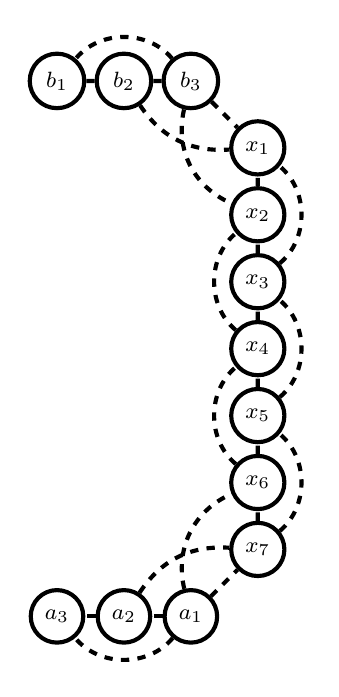
\begin{tikzpicture}[scale=0.85]
    \node[circle, draw=black, fill=white, line width=1.5pt, font=\footnotesize] (a2) at (0, 0) {$a_{3}$};
    \node[circle, draw=black, fill=white, line width=1.5pt, font=\footnotesize] (a1) at (1, 0) {$a_{2}$};
    \node[circle, draw=black, fill=white, line width=1.5pt, font=\footnotesize] (a0) at (2, 0) {$a_{1}$};

    \node[circle, draw=black, fill=white, line width=1.5pt, font=\footnotesize] (b2) at (0, 8) {$b_1$};
    \node[circle, draw=black, fill=white, line width=1.5pt, font=\footnotesize] (b1) at (1, 8) {$b_2$};
    \node[circle, draw=black, fill=white, line width=1.5pt, font=\footnotesize] (b0) at (2, 8) {$b_3$};
    
    \node[circle, draw=black, fill=white, line width=1.5pt, font=\footnotesize] (x1) at (3, 1) {$x_{7}$};
    \node[circle, draw=black, fill=white, line width=1.5pt, font=\footnotesize] (x2) at (3, 2) {$x_{6}$};
    \node[circle, draw=black, fill=white, line width=1.5pt, font=\footnotesize] (x3) at (3, 3) {$x_{5}$};
    \node[circle, draw=black, fill=white, line width=1.5pt, font=\footnotesize] (x4) at (3, 4) {$x_{4}$};
    \node[circle, draw=black, fill=white, line width=1.5pt, font=\footnotesize] (x5) at (3, 5) {$x_{3}$};
    \node[circle, draw=black, fill=white, line width=1.5pt, font=\footnotesize] (x6) at (3, 6) {$x_{2}$};
    \node[circle, draw=black, fill=white, line width=1.5pt, font=\footnotesize] (x7) at (3, 7) {$x_{1}$};
    
    \draw[line width=1.5pt, dashed] (a0) to (a1);
    \draw[line width=1.5pt, dashed] (a1) to (a2);
    \draw[line width=1.5pt, bend left=50, dashed] (a0) to (a2);

    \draw[line width=1.5pt, dashed] (b0) to (b1);
    \draw[line width=1.5pt, dashed] (b1) to (b2);
    \draw[line width=1.5pt, bend right=50, dashed] (b0) to (b2);


    \draw[line width=1.5pt, dashed] (x1) to (x2);
    \draw[line width=1.5pt, dashed] (x2) to (x3);
    \draw[line width=1.5pt, dashed] (x3) to (x4);
    \draw[line width=1.5pt, dashed] (x4) to (x5);
    \draw[line width=1.5pt, dashed] (x5) to (x6);
    \draw[line width=1.5pt, dashed] (x6) to (x7);

    \draw[line width=1.5pt, bend right=50, dashed] (x1) to (x3);
    \draw[line width=1.5pt, bend left=50, dashed] (x2) to (x4);
    \draw[line width=1.5pt, bend right=50, dashed] (x3) to (x5);
    \draw[line width=1.5pt, bend left=50, dashed] (x4) to (x6);
    \draw[line width=1.5pt, bend right=50, dashed] (x5) to (x7);

    \draw[line width=1.5pt, dashed] (a0) to (x1);
    \draw[line width=1.5pt, bend left=40, dashed] (a0) to (x2);
    \draw[line width=1.5pt, dashed, bend left=30,] (a1) to (x1);

    \draw[line width=1.5pt, dashed] (b0) to (x7);
    \draw[line width=1.5pt, bend right=40, dashed] (b0) to (x6);
    \draw[line width=1.5pt, dashed, bend right=30] (b1) to (x7);
\end{tikzpicture}
        \end{figure}
    \end{column}
\end{columns}
\end{frame}


%--------------------------------------------

% \begin{frame}{}
%     We now have \((r-1) \cdot (3k-2)\) vertices.\\
%     Vertices connected paths of length \(n-3\) in configuration graph \\
%     Each connection adds \(4k-2\) vertices\\
%     Configuration graph has now diameter
%     \vspace{-1em}
%     \[(4k-2)(r-1)+\sum d_i\]
%     \begin{columns}
%     \begin{column}{0.6\textwidth}
%         We can use a shortcut to skip \(b_1\) altogether.\\
%         Symmetrically we can do the same on the other side skipping \(a_3\).\\
%         \only<7>{
%         Thus we reduced each connection by 2.\\
%         Finally we obtain:
%             \[(4k-4)(r-1)+\sum d_i\]
%         }
%     \end{column}
%     \begin{column}{0.4\textwidth}
%     \begin{figure}
%         \centering
%         \only<1-2>{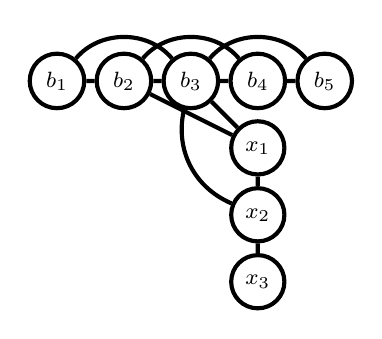
\begin{tikzpicture}[scale=0.85]

    \node[circle, draw=black, fill=white, line width=1.5pt, font=\footnotesize] (b2) at (0, 2) {$b_1$};
    \node[circle, draw=black, fill=white, line width=1.5pt, font=\footnotesize] (b1) at (1, 2) {$b_2$};
    \node[circle, draw=black, fill=white, line width=1.5pt, font=\footnotesize] (b0) at (2, 2) {$b_3$};
    
    \node[circle, draw=black, fill=white, line width=1.5pt, font=\footnotesize] (x5) at (3, -1) {$x_{3}$};
    \node[circle, draw=black, fill=white, line width=1.5pt, font=\footnotesize] (x6) at (3, 0) {$x_{2}$};
    \node[circle, draw=black, fill=white, line width=1.5pt, font=\footnotesize] (x7) at (3, 1) {$x_{1}$};
    

    \draw[line width=1.5pt] (b0) to (b1);
    \draw[line width=1.5pt] (b1) to (b2);
    \draw[line width=1.5pt, bend right=50] (b0) to (b2);


    \draw[line width=1.5pt] (x5) to (x6);
    \draw[line width=1.5pt] (x6) to (x7);

    \draw[line width=1.5pt] (b0) to (x7);
    \draw[line width=1.5pt, bend right=40] (b0) to (x6);
    \draw[line width=1.5pt] (b1) to (x7);
    
    \onslide<2>{
        \node[circle, draw=black, fill=white, line width=1.5pt, font=\footnotesize] (b3) at (3, 2) {$b_4$};
        \node[circle, draw=black, fill=white, line width=1.5pt, font=\footnotesize] (b4) at (4, 2) {$b_5$};
        \draw[line width=1.5pt] (b0) to (b3);
        \draw[line width=1.5pt] (b3) to (b4);
        \draw[line width=1.5pt, bend left=50] (b1) to (b3);
        \draw[line width=1.5pt, bend left=50] (b0) to (b4);
    }
\end{tikzpicture}
}
\only<3>{\begin{tikzpicture}[scale=0.85]

    \node[circle, draw=black, fill=white, line width=1.5pt, font=\footnotesize] (b2) at (0, 2) {$b_1$};
    \node[circle, draw=black, fill=white, line width=1.5pt, font=\footnotesize] (b1) at (1, 2) {$b_2$};
    \node[circle, draw=black, fill=cfred, line width=1.5pt, font=\footnotesize] (b0) at (2, 2) {$b_3$};
    
    \node[circle, draw=black, fill=white, line width=1.5pt, font=\footnotesize] (x5) at (3, -1) {$x_{3}$};
    \node[circle, draw=black, fill=white, line width=1.5pt, font=\footnotesize] (x6) at (3, 0) {$x_{2}$};
    \node[circle, draw=black, fill=white, line width=1.5pt, font=\footnotesize] (x7) at (3, 1) {$x_{1}$};
    

    \draw[line width=1.5pt] (b0) to (b1);
    \draw[line width=1.5pt] (b1) to (b2);
    \draw[line width=1.5pt, bend right=50] (b0) to (b2);


    \draw[line width=1.5pt] (x5) to (x6);
    \draw[line width=1.5pt] (x6) to (x7);

    \draw[line width=1.5pt] (b0) to (x7);
    \draw[line width=1.5pt, bend right=40] (b0) to (x6);
    \draw[line width=1.5pt] (b1) to (x7);
    
        \node[circle, draw=black, fill=cfred, line width=1.5pt, font=\footnotesize] (b3) at (3, 2) {$b_4$};
        \node[circle, draw=black, fill=cfred, line width=1.5pt, font=\footnotesize] (b4) at (4, 2) {$b_5$};
        \draw[line width=1.5pt] (b0) to (b3);
        \draw[line width=1.5pt] (b3) to (b4);
        \draw[line width=1.5pt, bend left=50] (b1) to (b3);
        \draw[line width=1.5pt, bend left=50] (b0) to (b4);
\end{tikzpicture}
}
\only<4>{\begin{tikzpicture}[scale=0.85]

    \node[circle, draw=black, fill=white, line width=1.5pt, font=\footnotesize] (b2) at (0, 2) {$b_1$};
    \node[circle, draw=black, fill=cfred, line width=1.5pt, font=\footnotesize] (b1) at (1, 2) {$b_2$};
    \node[circle, draw=black, fill=cfred, line width=1.5pt, font=\footnotesize] (b0) at (2, 2) {$b_3$};
    
    \node[circle, draw=black, fill=white, line width=1.5pt, font=\footnotesize] (x5) at (3, -1) {$x_{3}$};
    \node[circle, draw=black, fill=white, line width=1.5pt, font=\footnotesize] (x6) at (3, 0) {$x_{2}$};
    \node[circle, draw=black, fill=white, line width=1.5pt, font=\footnotesize] (x7) at (3, 1) {$x_{1}$};
    

    \draw[line width=1.5pt] (b0) to (b1);
    \draw[line width=1.5pt] (b1) to (b2);
    \draw[line width=1.5pt, bend right=50] (b0) to (b2);


    \draw[line width=1.5pt] (x5) to (x6);
    \draw[line width=1.5pt] (x6) to (x7);

    \draw[line width=1.5pt] (b0) to (x7);
    \draw[line width=1.5pt, bend right=40] (b0) to (x6);
    \draw[line width=1.5pt] (b1) to (x7);
    
        \node[circle, draw=black, fill=cfred, line width=1.5pt, font=\footnotesize] (b3) at (3, 2) {$b_4$};
        \node[circle, draw=black, fill=cfred!20, line width=1.5pt, font=\footnotesize] (b4) at (4, 2) {$b_5$};
        \draw[line width=1.5pt] (b0) to (b3);
        \draw[line width=1.5pt] (b3) to (b4);
        \draw[line width=1.5pt, bend left=50] (b1) to (b3);
        \draw[line width=1.5pt, bend left=50] (b0) to (b4);
\end{tikzpicture}
}
\only<5>{\begin{tikzpicture}[scale=0.85]

    \node[circle, draw=black, fill=white, line width=1.5pt, font=\footnotesize] (b2) at (0, 2) {$b_1$};
    \node[circle, draw=black, fill=cfred, line width=1.5pt, font=\footnotesize] (b1) at (1, 2) {$b_2$};
    \node[circle, draw=black, fill=cfred, line width=1.5pt, font=\footnotesize] (b0) at (2, 2) {$b_3$};
    
    \node[circle, draw=black, fill=white, line width=1.5pt, font=\footnotesize] (x5) at (3, -1) {$x_{3}$};
    \node[circle, draw=black, fill=white, line width=1.5pt, font=\footnotesize] (x6) at (3, 0) {$x_{2}$};
    \node[circle, draw=black, fill=cfred, line width=1.5pt, font=\footnotesize] (x7) at (3, 1) {$x_{1}$};
    

    \draw[line width=1.5pt] (b0) to (b1);
    \draw[line width=1.5pt] (b1) to (b2);
    \draw[line width=1.5pt, bend right=50] (b0) to (b2);


    \draw[line width=1.5pt] (x5) to (x6);
    \draw[line width=1.5pt] (x6) to (x7);

    \draw[line width=1.5pt] (b0) to (x7);
    \draw[line width=1.5pt, bend right=40] (b0) to (x6);
    \draw[line width=1.5pt] (b1) to (x7);
    
        \node[circle, draw=black, fill=cfred!20, line width=1.5pt, font=\footnotesize] (b3) at (3, 2) {$b_4$};
        \node[circle, draw=black, fill=white, line width=1.5pt, font=\footnotesize] (b4) at (4, 2) {$b_5$};
        \draw[line width=1.5pt] (b0) to (b3);
        \draw[line width=1.5pt] (b3) to (b4);
        \draw[line width=1.5pt, bend left=50] (b1) to (b3);
        \draw[line width=1.5pt, bend left=50] (b0) to (b4);
\end{tikzpicture}
}
\only<6>{\begin{tikzpicture}[scale=0.85]

    \node[circle, draw=black, fill=white, line width=1.5pt, font=\footnotesize] (b2) at (0, 2) {$b_1$};
    \node[circle, draw=black, fill=cfred!20, line width=1.5pt, font=\footnotesize] (b1) at (1, 2) {$b_2$};
    \node[circle, draw=black, fill=cfred, line width=1.5pt, font=\footnotesize] (b0) at (2, 2) {$b_3$};
    
    \node[circle, draw=black, fill=white, line width=1.5pt, font=\footnotesize] (x5) at (3, -1) {$x_{3}$};
    \node[circle, draw=black, fill=cfred, line width=1.5pt, font=\footnotesize] (x6) at (3, 0) {$x_{2}$};
    \node[circle, draw=black, fill=cfred, line width=1.5pt, font=\footnotesize] (x7) at (3, 1) {$x_{1}$};
    

    \draw[line width=1.5pt] (b0) to (b1);
    \draw[line width=1.5pt] (b1) to (b2);
    \draw[line width=1.5pt, bend right=50] (b0) to (b2);


    \draw[line width=1.5pt] (x5) to (x6);
    \draw[line width=1.5pt] (x6) to (x7);

    \draw[line width=1.5pt] (b0) to (x7);
    \draw[line width=1.5pt, bend right=40] (b0) to (x6);
    \draw[line width=1.5pt] (b1) to (x7);
    
        \node[circle, draw=black, fill=white, line width=1.5pt, font=\footnotesize] (b3) at (3, 2) {$b_4$};
        \node[circle, draw=black, fill=white, line width=1.5pt, font=\footnotesize] (b4) at (4, 2) {$b_5$};
        \draw[line width=1.5pt] (b0) to (b3);
        \draw[line width=1.5pt] (b3) to (b4);
        \draw[line width=1.5pt, bend left=50] (b1) to (b3);
        \draw[line width=1.5pt, bend left=50] (b0) to (b4);
\end{tikzpicture}
}
\only<7>{\begin{tikzpicture}[scale=0.85]

    \node[circle, draw=black, fill=white, line width=1.5pt, font=\footnotesize] (b2) at (0, 2) {$b_1$};
    \node[circle, draw=black, fill=white, line width=1.5pt, font=\footnotesize] (b1) at (1, 2) {$b_2$};
    \node[circle, draw=black, fill=cfred!20, line width=1.5pt, font=\footnotesize] (b0) at (2, 2) {$b_3$};
    
    \node[circle, draw=black, fill=cfred, line width=1.5pt, font=\footnotesize] (x5) at (3, -1) {$x_{3}$};
    \node[circle, draw=black, fill=cfred, line width=1.5pt, font=\footnotesize] (x6) at (3, 0) {$x_{2}$};
    \node[circle, draw=black, fill=cfred, line width=1.5pt, font=\footnotesize] (x7) at (3, 1) {$x_{1}$};
    

    \draw[line width=1.5pt] (b0) to (b1);
    \draw[line width=1.5pt] (b1) to (b2);
    \draw[line width=1.5pt, bend right=50] (b0) to (b2);


    \draw[line width=1.5pt] (x5) to (x6);
    \draw[line width=1.5pt] (x6) to (x7);

    \draw[line width=1.5pt] (b0) to (x7);
    \draw[line width=1.5pt, bend right=40] (b0) to (x6);
    \draw[line width=1.5pt] (b1) to (x7);
    
        \node[circle, draw=black, fill=white, line width=1.5pt, font=\footnotesize] (b3) at (3, 2) {$b_4$};
        \node[circle, draw=black, fill=white, line width=1.5pt, font=\footnotesize] (b4) at (4, 2) {$b_5$};
        \draw[line width=1.5pt] (b0) to (b3);
        \draw[line width=1.5pt] (b3) to (b4);
        \draw[line width=1.5pt, bend left=50] (b1) to (b3);
        \draw[line width=1.5pt, bend left=50] (b0) to (b4);
\end{tikzpicture}
}
%     \end{figure}
%     \end{column}
%     \end{columns}

% \end{frame}

%--------------------------------------------

\begin{frame}{What did we prove?}
    \begin{lemma}{Gluing Lemma}
        Let \(k \geq 3\). Let \(G\) be a graph on \(n\) vertices whose \(k\)-configuration graph contains \(r\) connected components. Then, there exists a graph on at most \(n+(3k-2)\cdot (r-1)\) vertices whose configuration graph had diameter at least \((4k-2)(r-1)+\sum d_i\)
    \end{lemma}

\end{frame}

%--------------------------------------------

\begin{frame}{Recap}
    \begin{theorem}{Upper bound for k=3}
        \[D(n,3)=\Omega(n^2/e^{O(\sqrt{\log n})})\]
    \end{theorem}
    \begin{heading}{Summary of the proof:}
    \begin{itemize}
        \item We construct a graph whose reconfiguration graph is the disjoint union of \(n/e^{o(\sqrt{\log n})}\) paths of linear length by using 3-AP free sets.
        \item We proved that we can add not many vertices to this graph to connect it and make the diameter sum of the components.
    \end{itemize}
    \end{heading}
\end{frame}